% !TeX program = lualatex
\documentclass[aspectratio=169,t,xcolor=table]{beamer}

% Text encoding
% \usepackage{inputenc}
% \inputencoding{utf8}

% Language
%\usepackage{babel}
%\selectlanguage{english}

% Layout
\usepackage{adjustbox}

% Underline
\usepackage{ulem}

% Hyperlinks
\usepackage{hyperref}
\hypersetup{
  colorlinks=true,
  filecolor=magenta,
  urlcolor=cyan,
  citecolor=cyan,
  linkcolor=cyan
}

% Tables
\usepackage{booktabs}

% Math
\usepackage{amsmath}
\usepackage{amssymb}
\usepackage{bm}
\usepackage{siunitx}
\usepackage{mathtools}

% Unnumbered footnote
\let\svthefootnote\thefootnote%
\textheight 1in
\newcommand\blankfootnote[1]{%
  \let\thefootnote\relax\footnotetext{\tiny #1}%
  \let\thefootnote\svthefootnote%
}

% Tikz
\usepackage{tikz}
\usetikzlibrary{positioning,decorations.pathreplacing,quotes,overlay-beamer-styles}

% Make it nicer
\usepackage{emoji}

% References
%\usepackage[natbib=true]{biblatex}
%\addbibresource{references.bib}
%\usepackage{natbib}

% Presentation settings
\mode<presentation>
{
  \usetheme{default}
  \usecolortheme{default}
  \usefonttheme{default}
  \setbeamertemplate{caption}

  % Theme hacking
  %% Default margin: 1cm
  \setbeamersize{text margin left=0.5cm, text margin right=0.5cm}

  %% Footer
  \setbeamerfont{footline}{size=\fontsize{3}{0}\selectfont}
  \setbeamercolor{section in head/foot}{fg=white, bg=ISUcardinal}
  %%% https://tex.stackexchange.com/a/111466/225233
  \setbeamertemplate{footline}
  {
    \hypersetup{allcolors=.}
    \leavevmode%
    \hbox{%
      \begin{beamercolorbox}[wd=.2\paperwidth,ht=2.25ex,dp=1ex,left]{section
	  in head/foot}%
	\usebeamerfont{author in head/foot}\insertshortauthor{}
      \end{beamercolorbox}%
      \begin{beamercolorbox}[wd=.6\paperwidth,ht=2.25ex,dp=1ex,center]{section
	  in head/foot}%
	  \usebeamerfont{title in head/foot}\insertshorttitle{}
	% \usebeamerfont{title in head/foot}Automatic Dynamic
	% Relevance Determination
      \end{beamercolorbox}%
      \begin{beamercolorbox}[wd=.2\paperwidth,ht=2.25ex,dp=1ex,right]{section
	  in head/foot}%
	\usebeamerfont{date in head/foot}\insertshortdate{}\hspace*{2em}
	\insertframenumber{} / \inserttotalframenumber\hspace*{2ex}
      \end{beamercolorbox}}%
    \vskip0pt%
  }

  %% Hide navigation bar
  \beamertemplatenavigationsymbolsempty{}

  %% ISU colors
  \definecolor{ISUcardinal}{RGB}{200,16,46}
  \definecolor{ISUgold}{RGB}{241,190,72}
  \definecolor{ISUgray}{RGB}{82,71,39}
  \definecolor{ISUsand}{RGB}{155,148,95}
  \definecolor{ISUgreen}{RGB}{202,199,167}

  %% Title page
  \setbeamercolor*{title}{fg=ISUcardinal}

  %% Frame
  \setbeamercolor{frametitle}{fg=white, bg=ISUcardinal}

  %% Lists
  \setbeamertemplate{itemize item}[square]
  \setbeamertemplate{itemize subitem}[triangle]
  \setbeamertemplate{itemize subsubitem}[triangle]

  \setbeamercolor{itemize item}{fg=ISUcardinal}
  \setbeamercolor{itemize subitem}{fg=ISUcardinal}
  \setbeamercolor{itemize subsubitem}{fg=ISUcardinal}

  \setbeamercolor{description item}{fg=ISUcardinal}

  %\setlength{\leftmargini}{0pt}
  \setlength{\leftmarginii}{10pt}
}

\usepackage{DejaVuSerif}
\usepackage[T1]{fontenc}

\newcommand\myHearts[1]{
  {
    \setbeamercolor{background canvas}{bg=ISUcardinal}
    \setbeamercolor{normal text}{fg=ISUgold}
    \begin{frame}
      \begin{tikzpicture}[overlay, remember picture]
	\node[anchor=center] at (current page.center) {
	  \begin{beamercolorbox}[center]{title}
	    \Huge
	    \color{ISUgold}
	    #1
	  \end{beamercolorbox}};
      \end{tikzpicture}
    \end{frame}
  }
}

% Setup
\graphicspath{{include/}}

\title{\textbf{Automatic Dynamic Relevance Determination} \\
  % of atmospheric states over vertical pressure grids \\
  for Gaussian process regressions with functional inputs}

\renewcommand*{\thefootnote}{\fnsymbol{footnote}}
\author[Damiano et al]{
  \textbf{Luis Damiano}\footnote[2]{
    \tiny{\href{mailto:ldamiano@iastate.edu}{ldamiano@iastate.edu}}
  }\inst{1}, Joaquim Teixeira\inst{2}, Margaret Johnson\inst{2}, Jarad Niemi\inst{1}}

\institute{
  \inst{1}Department of Statistics, Iowa State University \\
  \inst{2}NASA Jet Propulsion Laboratory
}

\date[April 13th, 2022]{\tiny{SIAM Conference on Uncertainty Quantification}\\ April 13th, 2022}

\begin{document}

% Title page
\begin{frame}
  \titlepage{}
  % \vspace{0.1in}
  {
    \tiny{
      Funded, in part, by
      \begin{itemize}
      \item[-] ISU Presidential Interdisciplinary
	Research Initiative on C-CHANGE:~Science for a Changing
	Agriculture
      \item[-] Foundation for Food and Agriculture Research
	Grant ID: CA18-SS-0000000278
      \end{itemize}
    }
  }
\end{frame}

% Introduction -----------------------------------------------------------------
\renewcommand{\thefootnote}{[\arabic{footnote}]}
\myHearts{Overview \& motivation}

\begin{frame}
  \frametitle{Gaussian process with functional input}
  \begin{tikzpicture}
    [
    txtbox1/.style={rectangle,align=center,draw=blue!50,fill=blue!20,thick},
    txtbox2/.style={rectangle,align=center,draw=red!50,fill=red!20,thick},
    every label/.style={font=\itshape\tiny}
    ]

    \node (inp)  [txtbox1] at ( 0,  0) [text width=16ex] {
      Functional input \\
      $X(t): \mathcal{T} \to \mathbb{R}$
    };
    \visible<2->{
      \node (vec1) [txtbox1] [above right=4ex of inp]   [text width=20ex]
      [label=below:No structural information]{
	As a vector \\
	$\mathbf{x} \in \mathbb{R}^K, K \in \mathbb{N}$
      };
      \node (vec2) [txtbox1] [below right=4ex of inp]   [text width=20ex]
      [label=above:Additional modeling decisions]{
	Basis representation \\
	$\tilde{\mathbf{x}} \in \mathbb{R}^K, K \in \mathbb{N}$
      };
    }
    \visible<3->{
      \node (dred) [txtbox1] [above right=4ex of vec2] [text width=10ex]
      [label=left:Many parameters]
      {
	Dimension \\ reduction
      };
    }

    \node (gp)   [txtbox2] [right=4ex of dred] [text width=10ex] {
      Gaussian \\ process
    };
    \node (out)  [txtbox2] [right=4ex of gp] [text width=10ex]  {
      Output \\ $y \in \mathbb{R}$
    };
    \visible<5->{
      \node [below=6ex of vec2.north, label=below:All this happens outside the GP$~^{[1]}$] {
      };
    }
    \draw [->] [visible on=<2->] (inp.north) |- (vec1.west);
    \draw [->] [visible on=<2->] (inp.south) |- (vec2.west);
    \draw [->] [visible on=<3->] (vec1.east) -| (dred.north);
    \draw [->] [visible on=<3->] (vec2.east) -| (dred.south);
    \draw [->] [visible on=<3->] (dred.east) -- (gp.west);
    \draw [->] (gp.east)   -- (out.west);
    \path [visible on=<5->] (inp.south west)
    edge[decorate,decoration={brace,mirror,raise=10ex},line width=.6pt]
    (inp.south west -| dred.south east);
  \end{tikzpicture}

  \begin{itemize}
  \item<4-> Can we connect the functional input structure to a physical
    mechanism?
  \item<5-> Can we incorporate the functional input structure into the GP?$~^{[2]}$
  \item<6-> Can we circumvent input dimension reduction?
  \end{itemize}

  \blankfootnote{\visible<5->{
      $~^{[1]}$\cite{muehlenstaedt2017,nanty2016,wang2017,tan2019,wang2019,betancourt2020,betancourt2020a,li2021} \,
      $~^{[2]}$\cite{morris2012,kuttubekova2019}
    }}
\end{frame}

\begin{frame}
  \frametitle{Input structure information}
  \begin{table}[]
    \footnotesize
    \begin{tabular}{@{}lllll@{}}
      \toprule
      \small Output
      & \begin{tabular}[c]{@{}l@{}}\small Input\\ $X(t): \mathcal{T} \to
	  \mathbb{R}$\end{tabular}
      & \begin{tabular}[c]{@{}l@{}}\small Index\\ $t \in \mathcal{T}$\end{tabular}
      & \begin{tabular}[c]{@{}l@{}}\small Index subspaces\\ $t \in
	  \mathcal{T}_u$\end{tabular}
      & \small Mechanism \\ \midrule
      \visible<2->{%
      Plant growth
      & Phosphorus
      & Depth
      & Soil layers
      & Root biomass \vspace{1ex}
      }
      \visible<3->{%
      \\
      & Precipitation
      & Time
      & Cycles, seasons
      &
	\begin{tabular}[c]{@{}l@{}}
	  Germination \\photosynthesis \\ nutrient absorption
	\end{tabular}
      \vspace{1ex}
      }
      \visible<4->{%
      \\
      Soil erosion
      & Elevation
      & Distance
      & Up/down slope
      & Water erosion \vspace{1ex}
      }
	\visible<5->{%
	\\
      Radiance
      & Chemical species
      & Elevation
      & Atmospheric layers
      & Reflectivity \vspace{0ex}
      }
      \\
      \bottomrule
    \end{tabular}
  \end{table}

  \vfill
  \begin{quote}<6->
    Index subspaces can provide a meaningful representation of the
    physical process
  \end{quote}

  \vfill
  \begin{quote}<7->
    Can we establish an explicit link $X(t) \xrightarrow{f} y$ for UQ?
  \end{quote}

\end{frame}

\myHearts{From relevance to \textit{dynamic} relevance}

\begin{frame}
  \frametitle{Extending relevance}

  \begin{tikzpicture}
    [
    txtbox1/.style={rectangle,align=center,draw=blue!50,fill=blue!20,thick},
    every label/.style={font=\itshape\footnotesize}
    ]
    \tikzset{every node/.style={align=center}}
    \node (prompt1)    at (0, 0)                       [text width=26ex]{
      Some inputs\\matter more than others\\
      $\mathbf{x}_1$ \textit{vs} $\mathbf{x}_2$
    };
    \node (prompt2)    [right=of prompt1]              [text
    width=26ex] [visible on=<2->]{
      Some index subspaces\\matter more than others\\
      $X(t_1)$ \textit{vs} $X(t_2)$
    };
    %%%%%
    \node (aspect1a)   [below left=of prompt1]         [text width=15ex] {
      Screening\\{\footnotesize \itshape (exploration \& diagnostics)}
    };
    \node (aspect1b)   [below=of aspect1a]             [text width=15ex] {
      Model tuning\\{\footnotesize \itshape (learning)}
    };
    %%%%%
    \node (solution1a) [below=of prompt1]              [text width=25ex] {
      Permutation\\Feature\\Importance$~^{[1]}$
    };
    \node (solution1b) [below=of solution1a]           [text width=25ex] {
      Automatic\\Relevance\\Determination$~^{[2]}$
    };
    %%%%%
    \node (solution2a) [txtbox1] [below=of prompt2]    [text
    width=25ex] [visible on=<3->]
    {
      Permutation\\Feature\\\textit{Dynamic Importance}$~^{[3]}$
    };
    \node (solution2b) [txtbox1] [below=of solution2a] [text
    width=25ex] [visible on=<4->]{
      Automatic\\\textit{Dynamic Relevance}\\Determination
    };
    \draw[shorten >=1ex,shorten <=2ex,line width=1pt] [->]
    [visible on=<2->] (prompt1.east) -- (prompt2.west);
    \draw[shorten >=2ex,shorten <=2ex,line width=1pt] [->]
    [visible on=<3->] (solution1a.east) -- (solution2a.west);
    \draw[shorten >=2ex,shorten <=2ex,line width=1pt] [->]
    [visible on=<4->] (solution1b.east) -- (solution2b.west);
  \end{tikzpicture}
  \blankfootnote{
    $~^{[1]}$~\cite{breiman2001,strobl2007,strobl2008,nicodemus2010,fisher2019,hooker2021}
    \,
    $~^{[2]}$~\cite{neal1996,piironen2016} \,
    \visible<3->{$~^{[3]}$ Forthcoming paper}
  }
  % \blankfootnote{$~^{[2]}$~\cite{neal1996,piironen2016}}
  % \blankfootnote{\visible<3->{$~^{[3]}$ Forthcoming paper}}
\end{frame}

\begin{frame}
  \frametitle{Modeling \textit{dynamic} relevance}
  \begin{tikzpicture}
    [
    txtbox1/.style={rectangle,align=center,draw=blue!50,fill=blue!20,thick},
    every label/.style={font=\itshape\footnotesize}
    ]
    \tikzset{every node/.style={align=center}}
    \node (aspect1b)   at (0, 0)                        [text width=15ex] {
      Model tuning\\{\footnotesize \itshape (learning)}
    };
    \node (aspect2)    [below=of aspect1b]              [text width=15ex] {
      Distance\\{\footnotesize $d(X_i, X_j)$}
    };
    \node (aspect3)    [below=of aspect2]               [text width=15ex] {
      Weights\\{\footnotesize \itshape (relevance)}
    };
    %%%%%
    \node (solution1b) [right=of aspect1b]              [text width=25ex] {
      Automatic\\Relevance\\Determination
    };
    %%%%%
    \node (solution2b) [txtbox1] [right=of solution1b]  [text
    width=25ex]
    [visible on=<2->]{
      Automatic\\\textit{Dynamic Relevance}\\Determination
    };
    %%%%%
    \node (eq1b) [below=of solution1b] [text width=25ex] {
      $\sum_{k=1}^K \frac{{(x_{i, k} - x_{j, k})}^2}{\ell_k^2}$
    };
    \node (eq2b) [below=of solution2b] [text width=25ex]
    [visible on=<3->]{
      $\int_{\mathcal{T}}
      \omega(t)
      {\left(X_i(t) - X_j(t) \right)}^2 \mathrm{d}t
      $
    };
    %%%%%
    \node (par1b) [below=of eq1b] [text width=25ex]{
      $\ell^{-2}_1, \cdots, \ell^{-2}_K > 0$
    };
    \node (par2b) [below=of eq2b] [text width=25ex]
    [visible on=<4->]{
      $\omega(t): \mathcal{T} \to \mathbb{R}^+$
    };
    \draw[shorten >=1ex,shorten <=1ex,line width=1pt]
    [visible on=<2->] [->] (solution1b.east) -- (solution2b.west);
    % \draw[shorten >=1ex,shorten <=1ex,line width=1pt]
    % [visible on=<3->] [->] (eq1b.east) -- (eq2b.west);
    % \draw[shorten >=1ex,shorten <=1ex,line width=1pt]
    % [visible on=<4->] [->] (par1b.east) -- (par2b.west);
  \end{tikzpicture}
\end{frame}

\begin{frame}
  \frametitle{Asymmetric Laplace function}

  \begin{columns}[t]
    \begin{column}{0.5\textwidth}
      \begin{align*}
	\omega(t)
	&= \text{exp}\left\{-(t - \tau) \lambda \kappa^s s\right\}
      \end{align*}
      \vspace{-5ex}
      \begin{figure}[h!]
	\centering
	  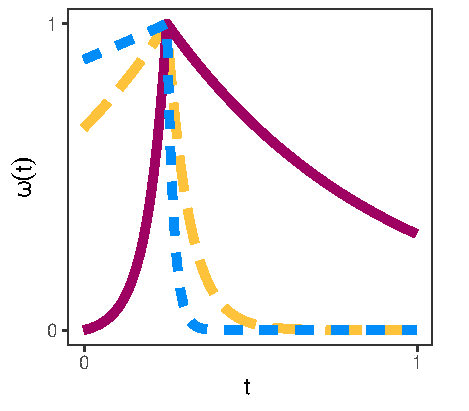
\includegraphics[width=.7\textwidth]{02-alf-weight-plot-ADE.pdf}%
      \end{figure}
    \end{column}
    \begin{column}{0.5\textwidth}
      \begin{itemize}
      \item<2-> The input is most relevant at $\tau$
	(relevance peak)
      \item<3-> Relevance increases at a $\lambda_1 = \lambda \kappa^{-1}$ rate
	from $t =0$ to the peak
      \item<4-> Relevance decreases at a $\lambda_2 = \lambda \kappa$ rate from
	the peak to $t = 1$
      \item<5-> To predict the output, look for input profiles that
	are similar everywhere \textit{but especially} near $\tau$
	\\ \visible<6->{\uwave{circumvent input dimension reduction}}
      \end{itemize}
    \end{column}
  \end{columns}

  \blankfootnote{
    $\omega(t): \mathcal{T} = [0, 1] \to (0, 1]$,
    $s = \text{sign}(t - \tau)$,
    $\tau > 0$,
    $\lambda > 0$,
    $\kappa > 0$
  }
\end{frame}

\begin{frame}{Functional Input Gaussian Process (fiGP)}
  \begin{align}
    \mathbf{y}
    &\sim \mathcal{N}\left(0, \sigma_{f}^{2} \ \mathbf{R}_f + \sigma_{\varepsilon}^{2}\mathbf{I}\right) \\
    {\left(\mathbf{R}_f\right)}_{ij}
    &=
      \text{exp}\left\{
      -0.5 \phi^{-2} \ d_f(X_i, X_j)
      \right\} \\
    \visible<2->{
    d_f(X_i, X_j)
    &= \int_{\mathcal{T}}
      \omega(t)
      {\left(X_i(t) - X_j(t) \right)}^2 dt
      } \\
    \visible<3->{
    \omega(t)
    &= \text{exp}\left\{-(t - \tau) \lambda \kappa^s s\right\}
      }
  \end{align}

  \blankfootnote{
    $\sigma_{\varepsilon}^2 > 0$,
    $\sigma_{f}^2 > 0$,
    $\phi > 0$,
    $i, j = 1, \dots, N$
  }

  \begin{description}
  \item[Weakly informative priors]<4-> $\phi \sim
    \textsc{InvGamma}$, $\tau \sim \textsc{Beta}$,
    $\lambda \sim \textsc{N}^{+}$, $\log(\kappa) \sim \textsc{N}$
  \item[Multiple inputs]<5-> e.g., correlation product
  \item[Complex index spaces]<6-> e.g., spatio-temporal spectral
    structures AKA tesseract
  \item[Flexibility]<7-> no need to match input-output structure nor index space
  \end{description}
\end{frame}

% Case study -------------------------------------------------------------------

\myHearts{NASA's Microwave Limb Sounder\\\footnotesize\textit{a case study}}

\begin{frame}
  \frametitle{Data structure}
  \begin{columns}[t]
    \begin{column}{0.5\textwidth}
      \begin{center}
	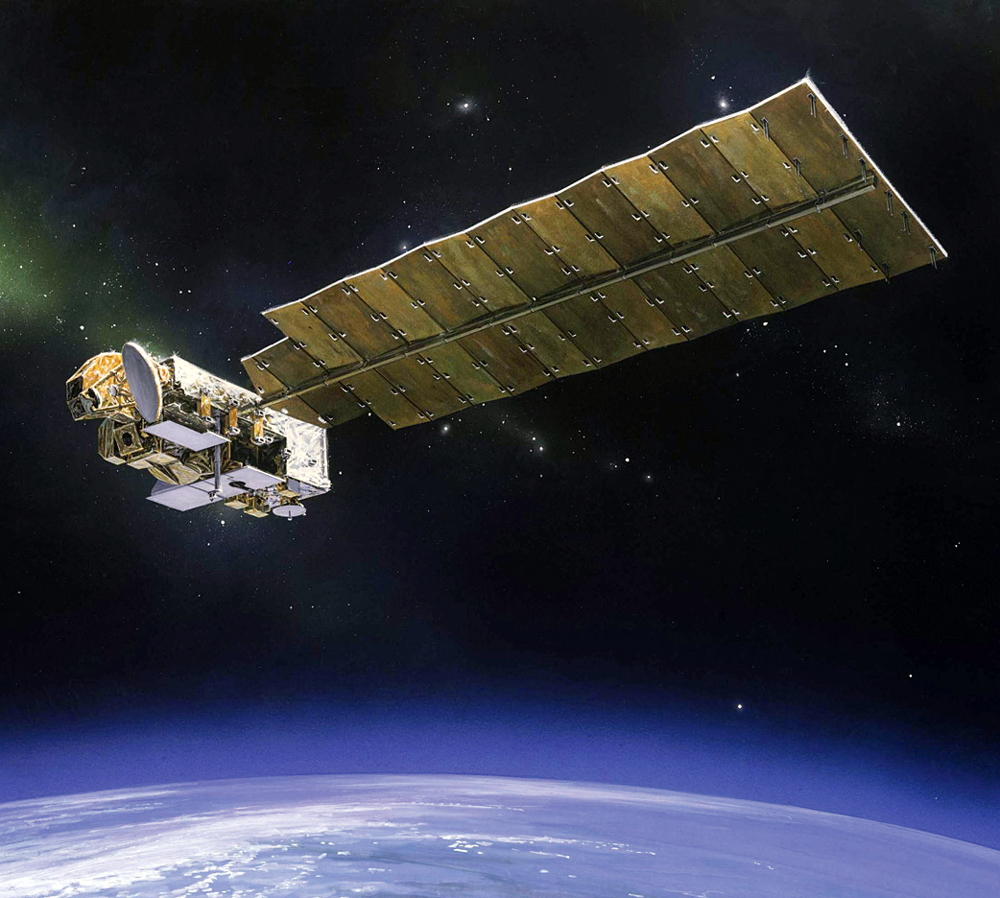
\includegraphics[height=.4\textheight]{aura.jpg}

	{\footnotesize \textit{Credit: NASA Aura}}

	\vspace{5ex}

	\definecolor{bright-spark}{RGB}{255, 195, 59}
	\tikzstyle{nice-rectangle} = [rectangle, rounded corners,
	minimum width=3cm, minimum height=1cm, text centered,
	draw=ISUcardinal, fill=bright-spark, font=\sffamily]
	\tikzset{every label/.style={font=\itshape\footnotesize}}
	\begin{tikzpicture}
	  \node (input) [nice-rectangle] [text width = 15ex] [label=below:Functional
	  input $X(t)$] {Atmospheric constituents};
	  \node
	  (output) [nice-rectangle, right=of input]
	  [label=below:Scalar output $y$] {Radiance};
	  \draw [->] (input) [above] -- node {$f$} (output);
	\end{tikzpicture}
      \end{center}
    \end{column}
    \begin{column}{0.5\textwidth}
      \begin{tikzpicture}[overlay, remember picture]
	\node[anchor=north west] (b) at (-.2, .9) {
	  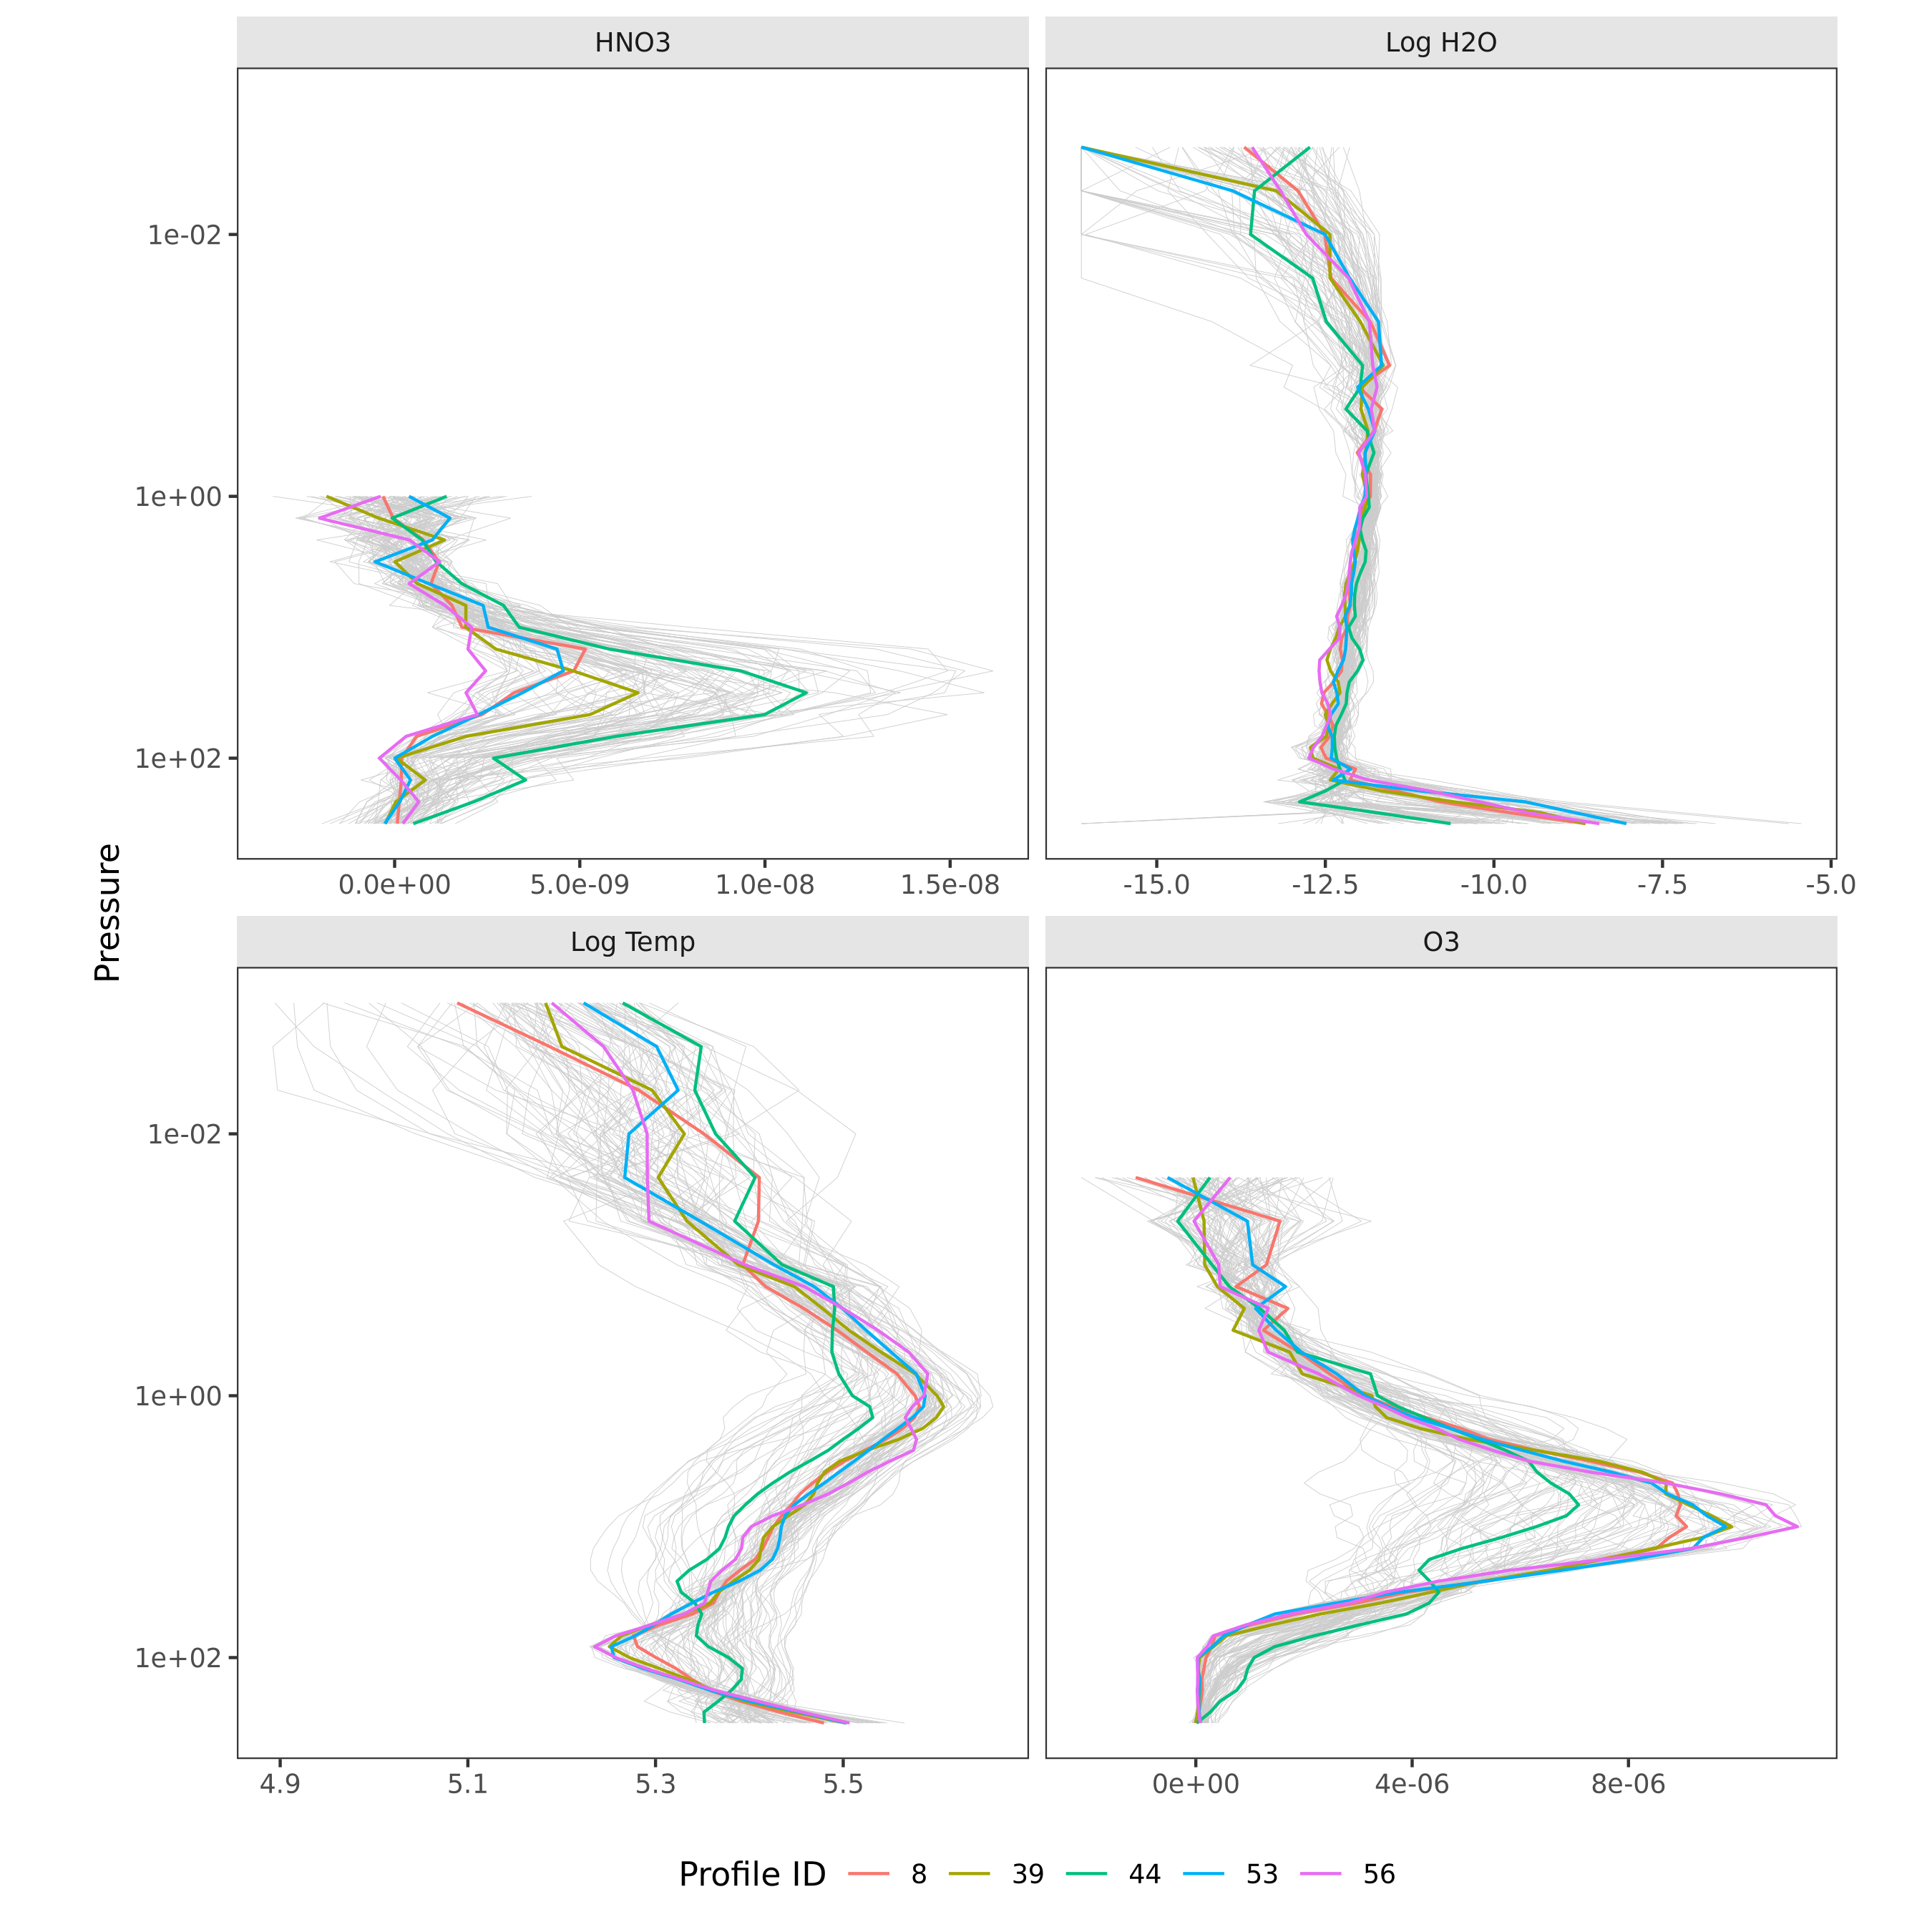
\includegraphics[height=.9\textheight]{eda-profile.png}
	};
      \end{tikzpicture}
    \end{column}
  \end{columns}
\end{frame}

\begin{frame}
  \frametitle{Implementation}
  \begin{itemize}
  \item 8 training, 8 test complementary sets
  \item 1,000 soundings each
  \item One model fit separately per input-output pair
  \item Fully Bayesian inference
  \item Hamiltonian Monte Carlo using Stan
  \item 1 long chain
  \item Extensive search for an initial value
  \item 500 post-warmup iterations
  \item 1,500 posterior samples
  \end{itemize}
\end{frame}

\begin{frame}
  \frametitle{Weight function posterior samples}

  \begin{figure}
    \centering
    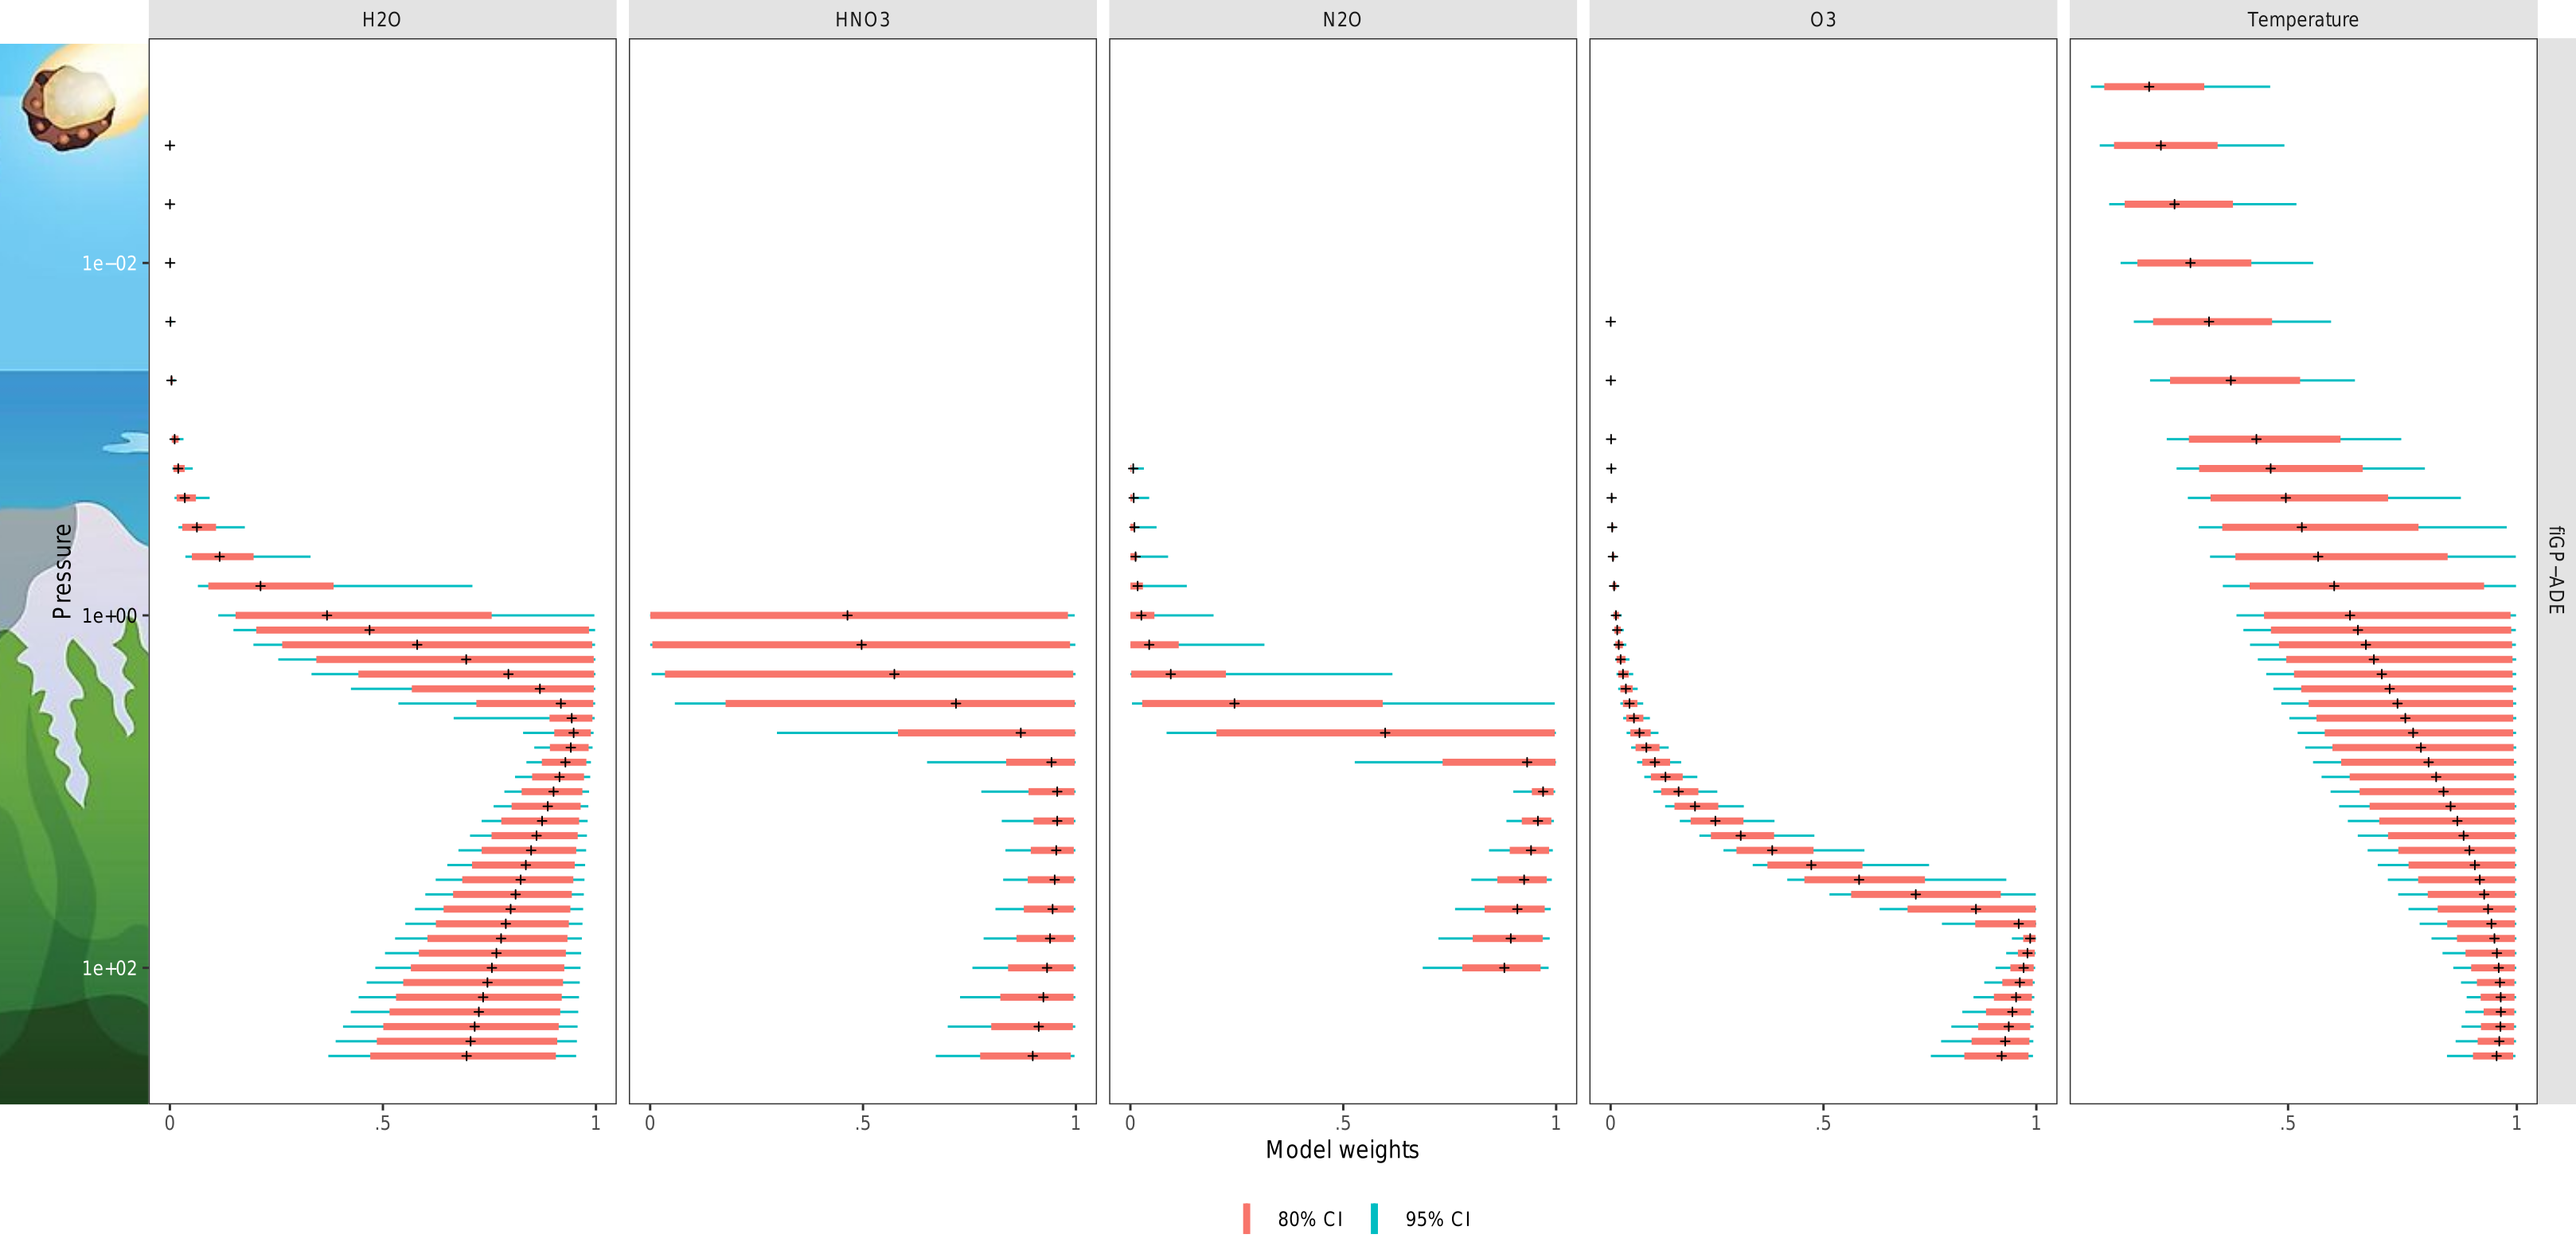
\includegraphics[width=1\textwidth]{image2934-8.png}
  \end{figure}
\end{frame}

\begin{frame}
  \frametitle{fiGP vs a vector-input GP}

  \begin{figure}
    \centering
    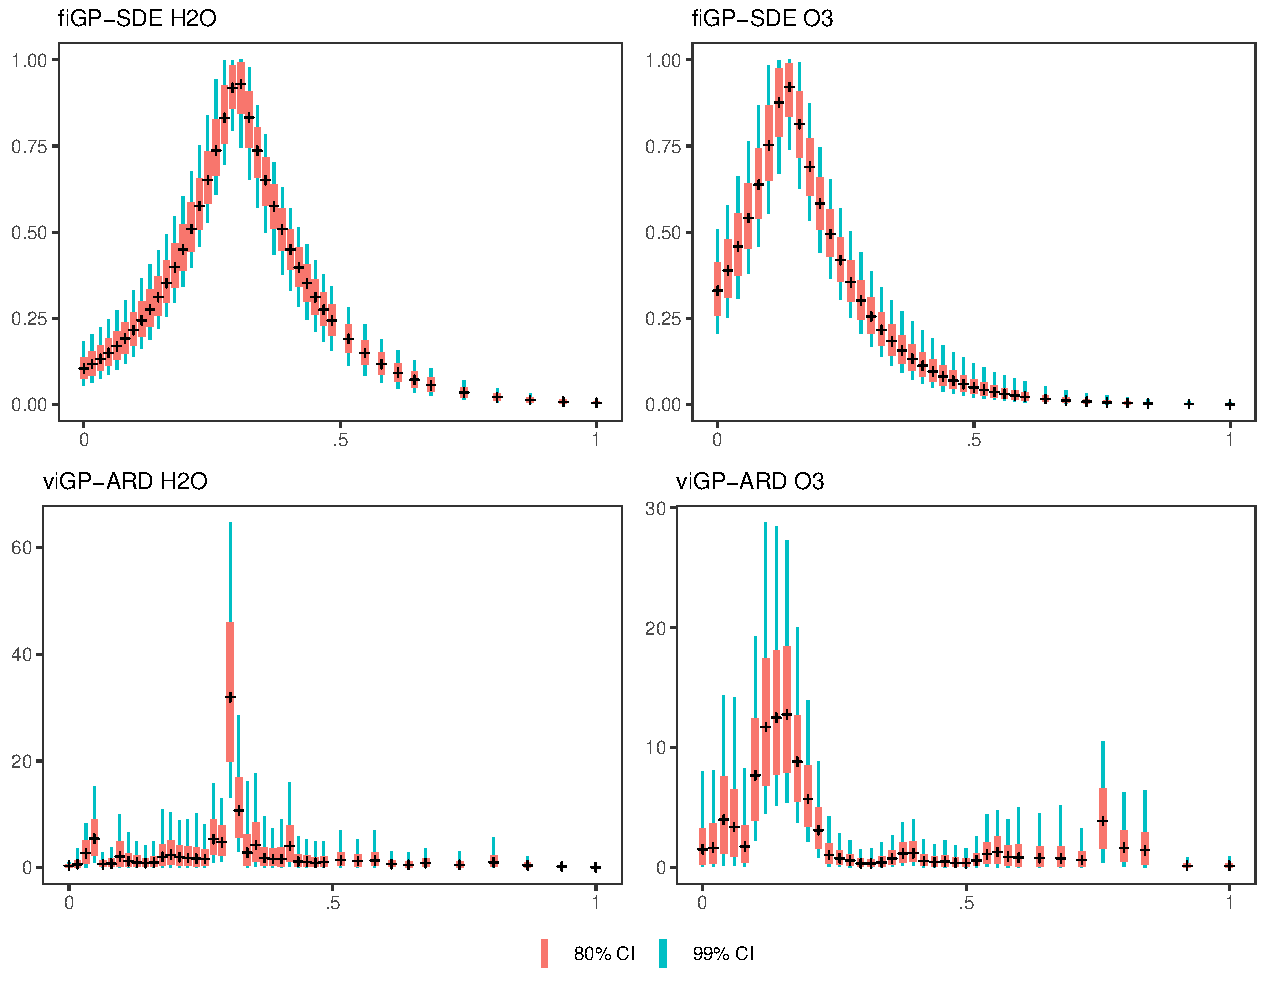
\includegraphics[height=.75\textheight]{weights-examples-pressure.pdf}
  \end{figure}

  \blankfootnote{In this slide only, we fix $\kappa = 1$ so that
    $\omega(t)$ is symmetrical}
\end{frame}

\begin{frame}
  \frametitle{Why a fiGP?}
  \begin{itemize}
  \item[+]<1-> High dimensional inputs with no dimension reduction
    \begin{itemize}
    \item Reduce unknowns $3 << K$
    \item Scales up for applications with higher input resolution
      $\uparrow K$
    \end{itemize}
  \item[+]<2-> Explicit link between output correlation and
    input functional structure
    \begin{itemize}
    \item<2-> Can incorporate domain-specific knowledge
    \item<2-> Tangible for prior elicitation
    \item<2-> Interpretation $\to$ insight?
    \item<2-> Smooths out erratic relevance patterns
    \end{itemize}
  \item[+]<3-> Similar predictive power as vector-input
    GP in the case study$~^{[1]}$
  \item[++]<4-> Extensible to \alert{\textbf{complex
index spaces}}, e.g., spatio-temporal spectral inputs$~^{[2]}$
\end{itemize}

\blankfootnote{
  \visible<3->{$~^{[1]}$~Appendix slides and forthcoming paper}%
  \visible<4->{\, $~^{[2]}$~Future research}
}
\end{frame}

\begin{frame}[c]
  \frametitle{Acknowledgments}
  \centering

  The MLS team at JPL, California Institute of Technology

  \vfill

  {\huge Thank you!}

  \vfill

  {\tiny References and extra slides on the back}

  \href{ldamiano@iastate.edu}{\beamergotobutton{mail}
    ldamiano@iastate.edu}

  \href{https://github.com/luisdamiano/SIAMUQ22}{\beamergotobutton{repo}
https://github.com/luisdamiano/SIAMUQ22}

\end{frame}

\myHearts{Appendix}

% % References -------------------------------------------------------------------
\section{References}

\setbeamertemplate{bibliography item}{\insertbiblabel}

\begin{frame}[allowframebreaks]{References}
  \tiny
  \bibliographystyle{unsrt}
  \bibliography{references}
\end{frame}

\begin{frame}{Notation}
    \only<1->{
    \begin{description}[labelwidth=117]
    \item[Index vector]<2-> $\mathbf{t}$ with the vertical pressure level
    \item[State vector]<3-> $\mathbf{x}_i$ characterizing an atmospheric
      vertical profile
    \item[Output scalar]<4-> $y_i$ is the radiance first
      functional principal component~\cite{johnson2020}
    \item[Sounding]<5-> a collection of an observed radiance, retrieved
      state and pressure vectors
    \end{description}
  }
\end{frame}

\begin{frame}
  \frametitle{Trapezoidal approximation}

  \begin{figure}[h!]
    \centering
    \caption[]{Trapezoidal approximation}
  \end{figure}

  {
    \setlength{\abovedisplayskip}{-1cm}
    \begin{align}
      \int_{\mathcal{T}}
      \omega(t)
      {\left(X_i(t) - X_j(t) \right)}^2 dt
      \approx
      &
      \sum_{k = 2}^{K} {
      \left(t_{k} - t_{k - 1}\right)
      \frac{
      \Delta_{i, j, k} +
      \Delta_{i, j, k - 1}
      }{2}
      } \\
      \Delta_{i, j, k} =
      & \
      \omega(t_{k-1}) {\left(x_{i, k} - x_{j, k}\right)}^2
    \end{align}
  }

  \blankfootnote{See~\cite{muehlenstaedt2017} for a B-spline
    approach}
\end{frame}

\begin{frame}
  \frametitle{Weights, inputs and output}

  \begin{figure}
    \centering
    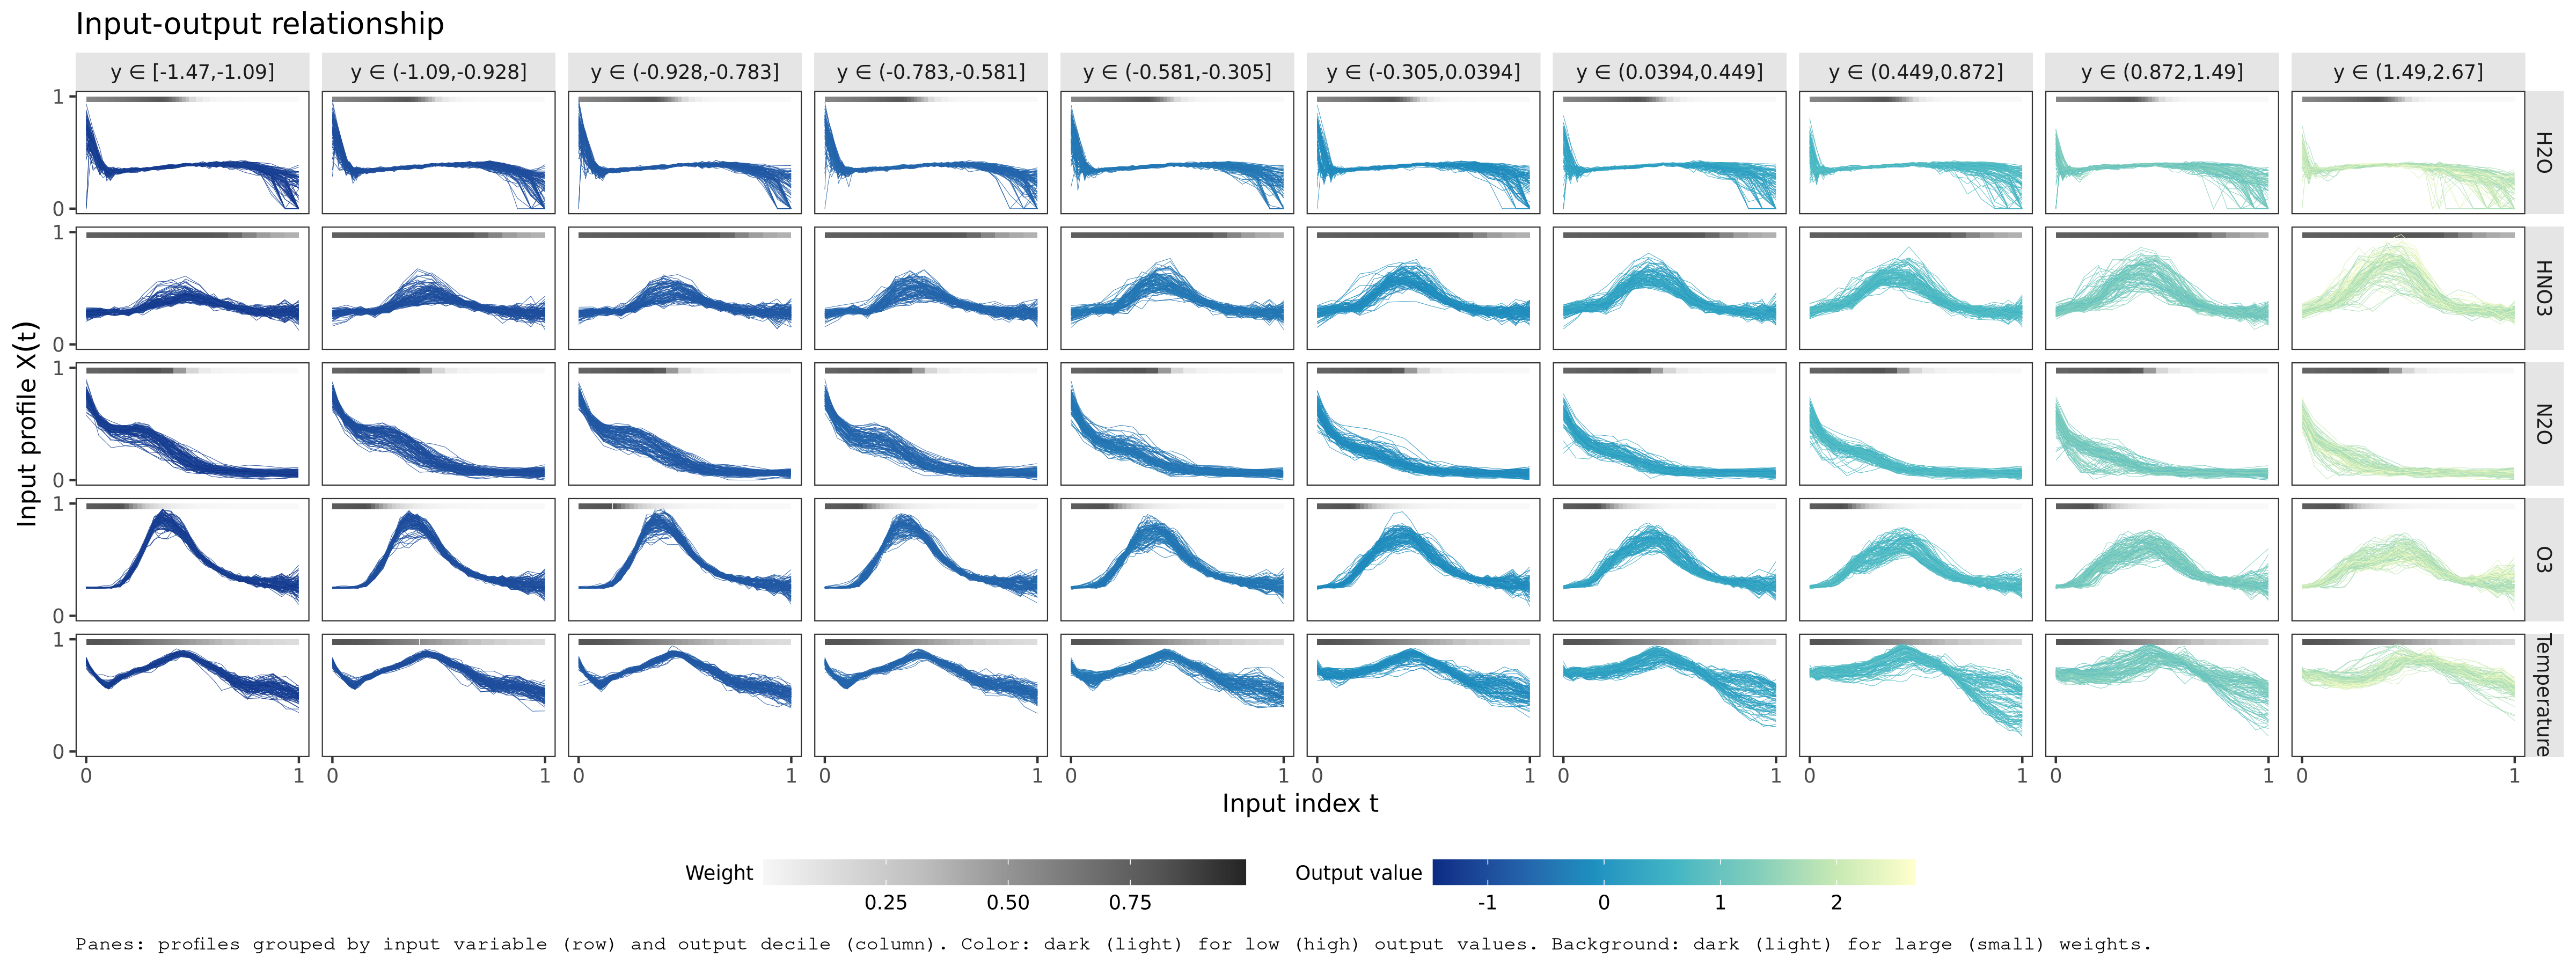
\includegraphics[width=1\textwidth]{io-lines-rug.png}
  \end{figure}
\end{frame}

\begin{frame}
  \frametitle{Out-of-sample prediction}
  \begin{table}
    \adjustbox{width=0.89\textwidth}{%
      \centering
      \begin{tabular}{lrrrrr|r}
	\toprule
	% latex table generated in R 4.0.4 by xtable 1.8-4 package
% Sat Dec 11 14:39:57 2021
%  & H2O & HNO3 & N2O & O3 & Temp & Mean \\ 
%   \midrule
% \textsc{SE} &  .34 &  .48 &  .44 &  .32 &  .25 &  .37 \\ 
%   \textsc{ARD} &  .31 &  .47 &  .43 &  .30 &  .25 &  .35 \\ 
%   \textsc{FPCA} &  .67 &  .91 &  .99 &  .46 &  .54 &  .71 \\ 
%   \textsc{FFPCA} &  .46 &  .54 &  .46 &  .38 &  .33 &  .44 \\ 
%   \textsc{Edn} &  .33 &  .47 &  .44 &  .29 &  .25 &  .36 \\ 
%   \textsc{SDE} &  .31 &  .47 &  .44 &  .29 &  .25 &  .35 \\ 
%   \textsc{ADE} &  .31 &  .47 &  .43 &  .29 &  .25 &  .35 \\ 
%    \midrule
% Mean &  .39 &  .55 &  .52 &  .33 &  .31 &  .42 \\ 
%    \bottomrule
 & H2O & HNO3 & N2O & O3 & Temp & Mean \\ 
  \midrule
  \textsc{SE}    &  .34       &  {\bf .48} &  {\bf .44} &  .32       &  {\bf .25} &  .37 \\ 
  \textsc{ARD}   &  {\bf .31} &  {\bf .47} &  {\bf .43} &  {\bf .30} &  {\bf .25} &  .35 \\ 
  \textsc{FPCA}  &  .67       &  .91       &  .99       &  .46       &  .54       &  .71 \\ 
  \textsc{FFPCA} &  .46       &  .54       &  {\bf .46} &  .38       &  .33       &  .44 \\ 
  \textsc{Edn}   &  .33       &  {\bf .47} &  {\bf .44} &  {\bf .29} &  {\bf .25} &  .36 \\ 
  \textsc{SDE}   &  {\bf .31} &  {\bf .47} &  {\bf .44} &  {\bf .29} &  {\bf .25} &  .35 \\ 
  \textsc{ADE}   &  {\bf .31} &  {\bf .47} &  {\bf .43} &  {\bf .29} &  {\bf .25} &  .35 \\ 
   \midrule
   Mean          &  .39 &  .55 &  .52 &  .33 &  .31 &  .42 \\ 
   \bottomrule
      \end{tabular}
      \begin{tabular}{lrrrrr|r}
	\toprule
	% latex table generated in R 4.0.4 by xtable 1.8-4 package
% Sat Dec 11 14:39:57 2021
  %                & H2O & HNO3 & N2O & O3 & Temp & Mean \\ 
  % \midrule
  % \textsc{SE}    & 273 & 613 & 589 & 142 & -4 & 323 \\ 
  % \textsc{ARD}   & 196 & 619 & 581 & 92 & -14 & 295 \\ 
  % \textsc{FPCA}  & 1024 & 1320 & 1406 & 637 & 802 & 1038 \\ 
  % \textsc{FFPCA} & 535 & 646 & 630 & 295 & 268 & 475 \\ 
  % \textsc{Edn}   & 260 & 623 & 585 & 90 & 4 & 312 \\ 
  % \textsc{SDE}   & 202 & 623 & 585 & 85 & 4 & 300 \\ 
  % \textsc{ADE}   & 202 & 610 & 581 & 89 & 2 & 297 \\ 
  %  \midrule
  %  Mean & 385 & 722 & 708 & 204 & 152 & 434 \\ 
  %  \bottomrule
                 & H2O & HNO3 & N2O & O3 & Temp & Mean \\ 
  \midrule
  \textsc{SE}    & 273       & {\bf 614} & {\bf 585} & 138      & {\bf -7}  & 323 \\ 
  \textsc{ARD}   & {\bf 196} & {\bf 619} & {\bf 581} & {\bf 92} & {\bf -13} & 295 \\ 
  \textsc{FPCA}  & 1024      & 1320      & 1406      & 637      & 802       & 1038 \\ 
  \textsc{FFPCA} & 535       & {\bf 646} & {\bf 630} & 295      & 268       & 475 \\ 
  \textsc{Edn}   & 261       & {\bf 623} & {\bf 585} & {\bf 90} & {\bf 4}   & 312 \\ 
  \textsc{SDE}   & {\bf 202} & {\bf 623} & {\bf 585} & {\bf 85} & {\bf 4}   & 300 \\ 
  \textsc{ADE}   & {\bf 202} & {\bf 610} & {\bf 581} & {\bf 87} & {\bf 2}   & 297 \\ 
   \midrule
   Mean & 385 & 722 & 708 & 204 & 152 & 434 \\ 
   \bottomrule
      \end{tabular}}
    \caption{Mean validation statistics
      $\bar{v}^{(p, q)}$: RMSE (left) and negPPLD (right).
      Smaller values are better. Bold: best in class.}%
    \label{tab:validation-statistics-mini}
  \end{table}

  Mean validation statistics: RMSE (left) and negative posterior
predictive log-density (right).  Smaller values are better. Bold: best
in column. \textsc{Edn} $\tau = 0, \kappa = 1$; \textsc{SDE} $\tau =
0$; \textsc{ADE} $\tau, \kappa, \lambda$ all free; \textsc{ARD} as
many free parameters as measurements per vertical profile.
\end{frame}

\end{document}

%%% Local Variables:
%%% mode: latex
%%% TeX-master: t
%%% End:
